% NeurReps 2026 poster -- A1 portrait (594 x 841 mm).
% Workshop cap is 610 mm (W) x 900 mm (H), so this fits with margin.
\documentclass[final,portrait]{beamer}
\usepackage[orientation=portrait,size=a1,scale=1.42]{beamerposter}
\usetheme{default}
\usepackage[utf8]{inputenc}
\usepackage[T1]{fontenc}
\usepackage{booktabs}
\usepackage{amsmath,amssymb}
\usepackage{graphicx}
\usepackage{xcolor}
\usepackage{tcolorbox}
\usepackage{qrcode}

\definecolor{ink}{HTML}{1A1A1A}
\definecolor{accent}{HTML}{C0392B}
\definecolor{pool}{HTML}{5D6D7E}
\definecolor{soft}{HTML}{F4F4F2}
\definecolor{rule}{HTML}{D8D8D4}

\setbeamercolor{background canvas}{bg=white}
\setbeamercolor{normal text}{fg=ink}
\setbeamerfont{normal text}{size=\normalsize}
\setbeamertemplate{navigation symbols}{}
\setbeamertemplate{caption}{\insertcaption}

% a plain block: coloured rule, bold heading, no box chrome
\newenvironment{psec}[1]{%
  \par\vspace{0.6em}%
  {\color{accent}\rule{\linewidth}{3pt}}\par\vspace{0.25em}%
  {\usebeamerfont*{frametitle}\bfseries\Large #1}\par\vspace{0.35em}%
}{\par\vspace{0.4em}}

\newcommand{\bignum}[2]{%
  \begin{minipage}[t]{\linewidth}\centering
  {\fontsize{64}{70}\selectfont\bfseries\color{accent}#1}\\[0.15em]
  {\large #2}
  \end{minipage}}

\begin{document}
\begin{frame}[t]{}
\vspace{-1.5em}

% ---------------- header ----------------
\begin{center}
{\fontsize{66}{74}\selectfont\bfseries Cortical Decoders Trained on Other\\[0.1em]
Individuals Age Slower Than Your Own}\\[0.7em]
{\LARGE Vihaan Shringi \quad\textperiodcentered\quad Carnegie Mellon University}\\[0.3em]
{\large NeurIPS 2026 Workshop on Symmetry and Geometry in Neural Representations}
\end{center}
\vspace{0.3em}
{\color{rule}\rule{\linewidth}{2pt}}
\vspace{0.6em}

\begin{columns}[t]

% ================= LEFT =================
\begin{column}{0.47\linewidth}

\begin{psec}{The question}
A decoder fit to one animal's cortex \textbf{drifts}: it loses accuracy on that same animal weeks
later. The standard remedy is recalibration --- collecting fresh labelled data from the subject,
over and over.

\vspace{0.4em}
Population structure is known to be \emph{shared} across individuals, and pooled decoders work.
But every one of those results is measured \textbf{at a single moment in time}.

\vspace{0.4em}
\textbf{Nobody had asked whether pooling resists drift.}
\end{psec}

\begin{psec}{The prediction}
A decoder that \emph{never saw} the subject cannot overfit that subject's drift-prone
idiosyncrasies --- so it should age more slowly. That difference is measurable as an
\textbf{asymmetry} between the two arms.
\end{psec}

\begin{psec}{Setup}
\textbf{BraiDyn-BC}: 25 mice, 44 Allen-atlas cortical parcels, widefield calcium, $\sim$15 daily
sessions over 3 weeks. Four task events decoded against matched negatives ($\ell_2$ logistic
regression, AUC).

\vspace{0.4em}
Per mouse, compare \textbf{aging} --- accuracy lost from an early block (days 1--5) to a late block
(days 11--15), training held fixed --- for a decoder trained on \textbf{itself} versus one
\textbf{pooled over the other 24 mice}.

\vspace{0.5em}
\begin{tcolorbox}[colback=soft,colframe=rule,boxrule=1pt,arc=2mm]
\textbf{Whole sessions are held out, not trials.} Only the within-subject arm can share a recording
session between train and test, so a trial-level split inflates \emph{that arm alone}.
\end{tcolorbox}
\end{psec}

\begin{psec}{The effect}
\vspace{0.2em}
\begin{center}
\bignum{$+0.017$}{AUC the personal decoder ages \emph{more}\\[0.2em]
$p = 5\times10^{-5}$ \quad\textperiodcentered\quad 73 of 100 mouse--event pairs}
\end{center}
\vspace{0.6em}

A day-by-day regression over all fifteen sessions agrees with the two-block contrast: the personal
decoder's early lead of $\sim$0.035 AUC narrows by $0.0014$/day ($p = 5\times10^{-5}$), so
\textbf{60\% of it is gone by day 15}.

\vspace{0.3em}
\begin{center}
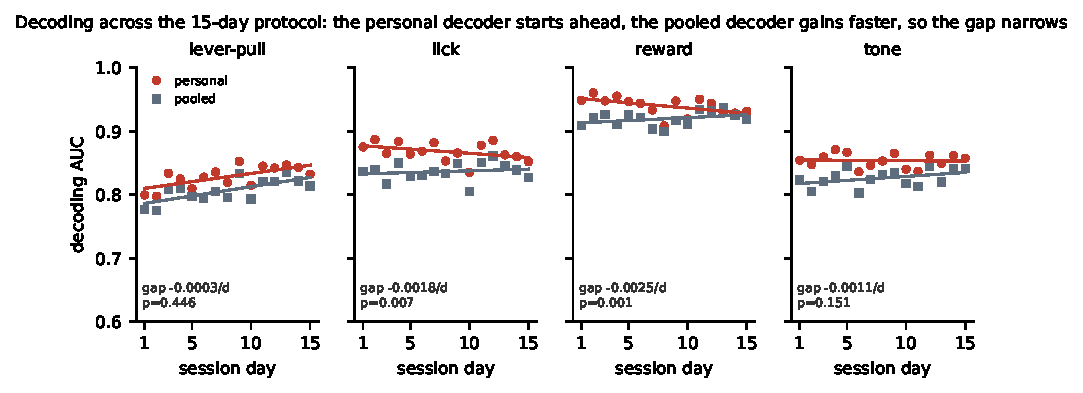
\includegraphics[width=0.99\linewidth]{fig_decay.pdf}
\end{center}
\vspace{0.1em}
{\small The pooled decoder \emph{gains} over days as the animal becomes more practised
($+0.0015$/day) while the personal decoder stays flat --- fit to idiosyncrasies, it cannot ride
that wave, and the lift it fails to take is what opens the gap.}
\end{psec}

\begin{psec}{Takeaway}
The early-week accuracy cost of decoding across individuals is \textbf{repaid as late-week
stability}. Population priors are a credible alternative to per-subject recalibration --- and they
need no new labelled data from the subject at deployment time, which is the expensive part.
\end{psec}

\end{column}

% ================= RIGHT =================
\begin{column}{0.47\linewidth}

\begin{psec}{Not a data-volume artifact}
A pooled decoder sees $\sim$24$\times$ more training events. So we fix the training-set size to $n$
and compare three decoders scored on identical held-out data.

\vspace{0.4em}
\begin{center}
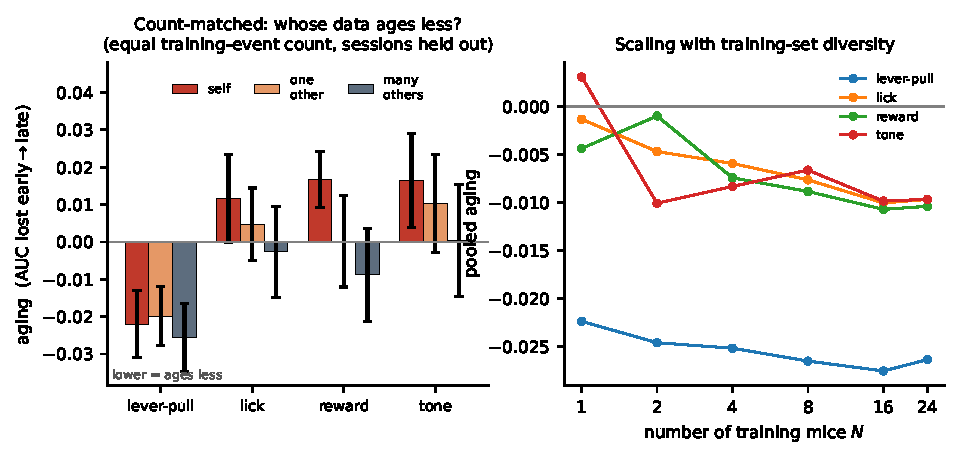
\includegraphics[width=0.99\linewidth]{fig_mechanism.pdf}
\end{center}
\vspace{0.2em}

At \textbf{equal data}, the subject's own decoder still ages most ($+0.010$ AUC vs.\ one other
mouse). Training on \emph{many} others beats \emph{one} other on all four events --- diversity adds
a further, smaller gain.
\end{psec}

\begin{psec}{It replicates on an independent cohort}
\vspace{0.3em}
{\centering
\begin{tabular}{lccc}
\toprule
& Asymmetry (95\% CI) & $p$ & own ages more \\
\midrule
BraiDyn-BC, widefield, 25 mice & $+0.017$ $[0.010,0.024]$ & $5\times10^{-5}$ & 73\% \\
Allen VB, two-photon, 23 mice  & $+0.023$ $[0.010,0.037]$ & $0.003$ & 74\% \\
\bottomrule
\end{tabular}\par}
\vspace{0.5em}

Different laboratory, cellular two-photon instead of mesoscale widefield, a visual change-detection
task instead of a cued lever pull, and a permutation-invariant population summary instead of an
atlas feature. \textbf{Little is shared but the question and the protocol.}

\vspace{0.4em}
The \emph{mechanism} differs: on BraiDyn-BC the gap narrows because the pooled decoder gains; here
because the personal decoder loses. The shared finding is that the personal decoder ages faster.
\end{psec}

\begin{psec}{Measuring it correctly}
\begin{tcolorbox}[colback=soft,colframe=accent,boxrule=2pt,arc=2mm]
Repeating the analysis with a \textbf{trial-level split} inflates the personal decoder's
within-block accuracy by up to $+0.013$ AUC and leaves the pooled decoder untouched.

\vspace{0.35em}
On lever pull that inflation is the \textbf{entire effect}:
$+0.014$ ($p=0.001$) $\;\rightarrow\;$ $+0.003$ ($p=0.37$).

\vspace{0.35em}
Any within- vs.\ cross-subject comparison is exposed to this. \textbf{Hold out sessions.}
\end{tcolorbox}
\end{psec}






\end{column}
\end{columns}

\vspace{0.3em}
{\color{rule}\rule{\linewidth}{2pt}}
\vspace{0.4em}
\begin{columns}[c]
\begin{column}{0.22\linewidth}
\centering\qrcode[height=2.6cm]{https://github.com/v1hns/braidyn-decoding}
\end{column}
\begin{column}{0.74\linewidth}
{\small \textbf{Code \& streamed-feature pipeline:} \texttt{github.com/v1hns/braidyn-decoding}\\
Both cohorts are public: DANDI:001425 and the Allen Brain Observatory.\\[0.3em]
\textit{Thanks to Vibha Singhal for detailed feedback on the structure and framing of an earlier
draft.}}
\end{column}
\end{columns}

\end{frame}
\end{document}
